%\documentclass{standalone}
%\usepackage{pgfplots} % Include package for TikZ and PGF plot
%\usepackage{anyfontsize} % enable to change the font size manually
%\usepackage{makecell}%
\usetikzlibrary{shapes.geometric}
\tikzset{
dot/.style = {circle, fill, minimum size=#1,
              inner sep=0pt, outer sep=0pt},
dot/.default = 6pt % size of the circle diameter 
}
 \renewcommand{\familydefault}{\sfdefault}

%\begin{document}
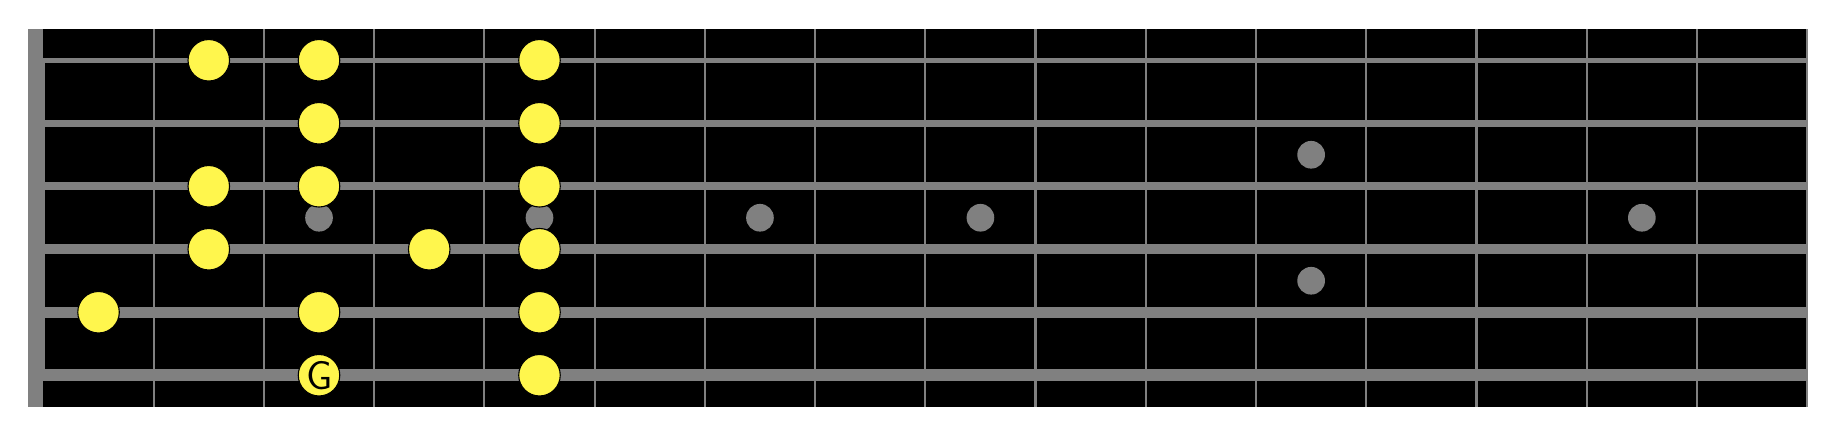
\begin{tikzpicture}[scale=1]
	\def \h{0.8}
	\def \fret{1.4} % 1.6
	\def \L{ 16*\fret }
	\def \dot_size{5pt}
	\def \circ_size{15pt}
	
	\fill[black, line width=2] (0.0,-0.4) rectangle (16*\fret,4.4);
	\fill[black!50!white, line width=2] (-0.2,-0.4) rectangle (0,4.4);
	
	% Strings
	\draw[color=black!50!white, line width=2.0]  (-0.1, 5*\h) -- (\L,5*\h); % E
	\draw[color=black!50!white, line width=2.5]  (-0.1, 4*\h) -- (\L,4*\h); % B
	\draw[color=black!50!white, line width=3.0]  (-0.1, 3*\h) -- (\L,3*\h); % G
	\draw[color=black!50!white, line width=3.5]  (-0.1, 2*\h) -- (\L,2*\h); % D
	\draw[color=black!50!white, line width=4.0]  (-0.1, 1*\h) -- (\L,1*\h); % A
	\draw[color=black!50!white, line width=4.5]  (-0.1, 0*\h) -- (\L,0*\h); % E
	
	% Frets 0
	\draw[color=black!50!white, thick]  (-0.1, 0) -- (-0.1,5*\h); 
	\draw[color=black!50!white, thick]  (0, 0)   -- (0,5*\h); 
	
	% Fret 1-15
	\draw[color=black!50!white, thick]  (\fret,   -0.4)   -- (\fret,4.4);   
	\draw[color=black!50!white, thick]  (2*\fret, -0.4) -- (2*\fret,4.4); 
	\draw[color=black!50!white, thick]  (3*\fret, -0.4) -- (3*\fret,4.4); 
	\draw[color=black!50!white, thick]  (4*\fret, -0.4) -- (4*\fret,4.4); 
	\draw[color=black!50!white, thick]  (5*\fret, -0.4) -- (5*\fret,4.4); 
	\draw[color=black!50!white, thick]  (6*\fret, -0.4) -- (6*\fret,4.4); 
	\draw[color=black!50!white, thick]  (7*\fret, -0.4) -- (7*\fret,4.4); 
	\draw[color=black!50!white, thick]  (8*\fret, -0.4) -- (8*\fret,4.4); 
	\draw[color=black!50!white, thick]  (9*\fret, -0.4) -- (9*\fret,4.4); 
	\draw[color=black!50!white, thick]  (10*\fret, -0.4) -- (10*\fret,4.4); 
	\draw[color=black!50!white, thick]  (11*\fret, -0.4) -- (11*\fret,4.4); 
	\draw[color=black!50!white, thick]  (12*\fret, -0.4) -- (12*\fret,4.4); 
	\draw[color=black!50!white, thick]  (13*\fret, -0.4) -- (13*\fret,4.4); 
	\draw[color=black!50!white, thick]  (14*\fret, -0.4) -- (14*\fret,4.4); 
	\draw[color=black!50!white, thick]  (15*\fret, -0.4) -- (15*\fret,4.4); 
	\draw[color=black!50!white, thick]  (16*\fret, -0.4) -- (16*\fret,4.4);
	
	% Dots
	\fill[black!50!white] (2.5*\fret,2.5*\h) circle (\dot_size); % fret 3
	\fill[black!50!white] (4.5*\fret,2.5*\h) circle (\dot_size); % fret 5
	\fill[black!50!white] (6.5*\fret,2.5*\h) circle (\dot_size); % fret 7
	\fill[black!50!white] (8.5*\fret,2.5*\h) circle (\dot_size); % fret 9
	\fill[black!50!white] (11.5*\fret,1.5*\h) circle (\dot_size); % fret 12
	\fill[black!50!white] (11.5*\fret,3.5*\h) circle (\dot_size); % fret 12
	\fill[black!50!white] (14.5*\fret,2.5*\h) circle (\dot_size); % fret 15
	
	% String names
%	\draw[black] (-0.5,5*\h) node { {\Large E} };
%	\draw[black] (-0.5,4*\h) node { {\Large B} };
%	\draw[black] (-0.5,3*\h) node { {\Large G} };
%	\draw[black] (-0.5,2*\h) node { {\Large D} };
%	\draw[black] (-0.5,1*\h) node { {\Large A} };
%	\draw[black] (-0.5,0*\h) node { {\Large E} };
	
	% Major scale (fret 1-5)
%	\node[dot=\circ_size, fill=yellow!70!white,draw] at (1.5*\fret,0) { };
	\node[dot=\circ_size, fill=yellow!70!white,draw] at (2.5*\fret,0) {\textcolor{black}{\Large G}};
	\node[dot=\circ_size, fill=yellow!70!white, draw] at (4.5*\fret,0) {};
	\node[dot=\circ_size, fill=yellow!70!white,draw] at (0.5*\fret,1*\h) {};
	\node[dot=\circ_size, fill=yellow!70!white,draw] at (2.5*\fret,1*\h) {};
	\node[dot=\circ_size, fill=yellow!70!white,draw] at (4.5*\fret,1*\h) {};

	\node[dot=\circ_size, fill=yellow!70!white,draw] at (1.5*\fret,2*\h) {};
	\node[dot=\circ_size, fill=yellow!70!white,draw] at (3.5*\fret,2*\h) {};
	\node[dot=\circ_size, fill=yellow!70!white,draw] at (4.5*\fret,2*\h) {};

	\node[dot=\circ_size, fill=yellow!70!white,draw] at (1.5*\fret,3*\h) {};
	\node[dot=\circ_size, fill=yellow!70!white,draw] at (2.5*\fret,3*\h) {};
	\node[dot=\circ_size, fill=yellow!70!white,draw] at (4.5*\fret,3*\h) {};

%	\node[dot=\circ_size, fill=white,draw] at (0.5*\fret,4*\h) {{\large C}};
	\node[dot=\circ_size, fill=yellow!70!white,draw] at (2.5*\fret,4*\h) {};
	\node[dot=\circ_size, fill=yellow!70!white,draw] at (4.5*\fret,4*\h) {};
	
	\node[dot=\circ_size, fill=yellow!70!white,draw] at (1.5*\fret,5*\h) {};
	\node[dot=\circ_size, fill=yellow!70!white,draw] at (2.5*\fret,5*\h) {};
	\node[dot=\circ_size, fill=yellow!70!white,draw] at (4.5*\fret,5*\h) {};
	
%	% Major scale (fret 7-10)
%	\node[dot=\circ_size, fill=cyan,draw] at (6.5*\fret,0)    {{\large B}};
%	\node[dot=\circ_size, fill=blue!50!white,draw] at (7.5*\fret,0)    {{\large C}};
%	\node[dot=\circ_size, fill=blue!50!red!50!white,draw] at (9.5*\fret,0)    {{\large D}};
%
%	\node[dot=\circ_size, fill=white,draw] at (6.5*\fret,1*\h) {{\large E}};
%	\node[dot=\circ_size, fill=white,draw] at (8.5*\fret,1*\h) {{\large {\normalsize F}{\tiny $^\#$}}};
%	\node[dot=\circ_size, fill=white,draw] at (9.5*\fret,1*\h) {{\large G}};
%
%	\node[dot=\circ_size, fill=white,draw] at (6.5*\fret,2*\h) {{\large A}};
%	\node[dot=\circ_size, fill=white,draw] at (8.5*\fret,2*\h) {{\large B}};
%	\node[dot=\circ_size, fill=white,draw] at (9.5*\fret,2*\h) {{\large C}};
%
%	\node[dot=\circ_size, fill=white,draw] at (6.5*\fret,3*\h) {{\large D}};
%	\node[dot=\circ_size, fill=white,draw] at (8.5*\fret,3*\h) {{\large E}};
%
%	\node[dot=\circ_size, fill=white,draw] at (6.5*\fret,4*\h) {{\large {\normalsize F}{\tiny $^\#$}}};
%	\node[dot=\circ_size, fill=white,draw] at (7.5*\fret,4*\h) {{\large G}};
%	\node[dot=\circ_size, fill=white,draw] at (9.5*\fret,4*\h) {{\large A}};
%
%	\node[dot=\circ_size, fill=white,draw] at (6.5*\fret,5*\h) {{\large B}};
%	\node[dot=\circ_size, fill=white,draw] at (7.5*\fret,5*\h) {{\large C}};
%	\node[dot=\circ_size, fill=white,draw] at (9.5*\fret,5*\h) {{\large D}};
%
%	% Major scale (fret 11-15)
%	\node[dot=\circ_size, fill=red!60!white,   draw] at (11.5*\fret,0)    {{\large E}};
%	\node[dot=\circ_size, fill=orange!80!white,draw] at (13.5*\fret,0)    {{\large {\normalsize F}{\tiny $^\#$}}};
%	\node[dot=\circ_size, fill=yellow!70!white,draw] at (14.5*\fret,0)    {{\large G}};
%
%	\node[dot=\circ_size, fill=white,draw] at (11.5*\fret,1*\h) {{\large A}};
%	\node[dot=\circ_size, fill=white,draw] at (13.5*\fret,1*\h) {{\large B}};
%	\node[dot=\circ_size, fill=white,draw] at (14.5*\fret,1*\h) {{\large C}};
%
%	\node[dot=\circ_size, fill=white,draw] at (11.5*\fret,2*\h) {{\large D}};
%	\node[dot=\circ_size, fill=white,draw] at (13.5*\fret,2*\h) {{\large E}};
%
%	\node[dot=\circ_size, fill=white,draw] at (10.5*\fret,3*\h) {{\large {\normalsize F}{\tiny $^\#$}}};
%	\node[dot=\circ_size, fill=white,draw] at (11.5*\fret,3*\h) {{\large G}};
%	\node[dot=\circ_size, fill=white,draw] at (13.5*\fret,3*\h) {{\large A}};
%
%	\node[dot=\circ_size, fill=white,draw] at (11.5*\fret,4*\h) {{\large B}};
%	\node[dot=\circ_size, fill=white,draw] at (12.5*\fret,4*\h) {{\large C}};
%	\node[dot=\circ_size, fill=white,draw] at (14.5*\fret,4*\h) {{\large D}};
%
%	\node[dot=\circ_size, fill=white,draw] at (11.5*\fret,5*\h) {{\large E}};
%	\node[dot=\circ_size, fill=white,draw] at (13.5*\fret,5*\h) {{\large {\normalsize F}{\tiny $^\#$}}};
%	\node[dot=\circ_size, fill=white,draw] at (14.5*\fret,5*\h) {{\large G}};
%
%	% Major scale (fret 16-20)
%	\node[dot=\circ_size, fill=white,draw] at (16.5*\fret,0) {{\large A}};
%	\node[dot=\circ_size, fill=white,draw] at (18.5*\fret,0) {{\large B}};
%	\node[dot=\circ_size, fill=white,draw] at (19.5*\fret,0) {{\large C}};
%
%	\node[dot=\circ_size, fill=white,draw] at (16.5*\fret,1*\h) {{\large D}};
%	\node[dot=\circ_size, fill=white,draw] at (18.5*\fret,1*\h) {{\large E}};
%
%	\node[dot=\circ_size, fill=white,draw] at (15.5*\fret,2*\h) {{\large {\normalsize F}{\tiny $^\#$}}};
%	\node[dot=\circ_size, fill=white,draw] at (16.5*\fret,2*\h) {{\large G}};
%	\node[dot=\circ_size, fill=white,draw] at (18.5*\fret,2*\h) {{\large A}};
%
%	\node[dot=\circ_size, fill=white,draw] at (15.5*\fret,3*\h) {{\large B}};
%	\node[dot=\circ_size, fill=white,draw] at (16.5*\fret,3*\h) {{\large C}};
%	\node[dot=\circ_size, fill=white,draw] at (18.5*\fret,3*\h) {{\large D}};
%
%	\node[dot=\circ_size, fill=white,draw] at (16.5*\fret,4*\h) {{\large E}};
%	\node[dot=\circ_size, fill=white,draw] at (18.5*\fret,4*\h) {{\large {\normalsize F}{\tiny $^\#$}}};
%	\node[dot=\circ_size, fill=white,draw] at (19.5*\fret,4*\h) {{\large G}};
%
%	\node[dot=\circ_size, fill=white,draw] at (16.5*\fret,5*\h) {{\large A}};
%	\node[dot=\circ_size, fill=white,draw] at (18.5*\fret,5*\h) {{\large B}};
%	\node[dot=\circ_size, fill=white,draw] at (19.5*\fret,5*\h) {{\large C}};
%
%	% Position 1 (ionien)
%	\draw [draw=yellow!90!black,         line width=2] (1.2*\fret,-0.5) rectangle (4.8*\fret,4.5);
%	% Position 2 (dorien)
%	\draw [draw=green!60!white!70!black, line width=2] (3.2*\fret,-0.7) rectangle (7.8*\fret,4.7);
%	% Position 3 (phrygien)
%	\draw [draw=cyan,                    line width=2] (6.2*\fret,-0.5) rectangle (9.8*\fret,4.5);
%	% Position 5 (mixolydien)
%	\draw [draw=blue!50!red!50!white,    line width=2] (8.2*\fret,-0.7) rectangle (12.8*\fret,4.7);
%	% Position 6 (eolien)
%	\draw [draw=red!60!white,            line width=2] (10.2*\fret,-0.5) rectangle (14.8*\fret,4.5);
	
	% Mode names
%	\draw[yellow!90!black,         anchor=center, text width=3.5cm, align=center] (3,-2.2) node { {\Large \textbf{Position~1 G~Ionian} }};
%	\draw[green!60!white!70!black, anchor=center, text width=3.5cm, align=center] (6.5,-2.2) node { {\Large \textbf{Position~2 A~Dorian} }};
%	\draw[cyan,                    anchor=center, text width=3.5cm, align=center] (9.5,-2.2) node { {\Large \textbf{Position~3 B~Phrygian} }};
%	\draw[blue!50!white,           anchor=center, text width=3.5cm, align=center] (11,-1.3) node { {\Large \textbf{Position~4 C~Lydian} }};
%	\draw[blue!50!red!50!white,    anchor=center, text width=3.5cm, align=center] (13.5,-2.2) node { {\Large \textbf{Position~5 D~Mixolydian} }};
%	\draw[red!60!white,            anchor=center, text width=3.5cm, align=center] (16.5,-2.2) node { {\Large \textbf{Position~6 E~Aeolian} }};
%	\draw[orange!80!white,         anchor=center, text width=3.5cm, align=center] (19.5,-2.2) node { {\Large \textbf{Position~7 F $^\#$~Locrian} }};
\end{tikzpicture}
%\end{document}